% =====================================================================
%  ch05.tex —— 第 5 章 微分形式与 de Rham 上同调（原书 p.74–88）
%  p.74 上半为第 4 章末（§4.7.3 与 Question 4.74–4.76），按 Lead 分块归入本文件。
%  §5.1 微分形式  §5.2 拉回与微分形式的积分  §5.3 de Rham 上同调
%  §5.4 de Rham 上同调的例子  §5.5 联络与 Maxwell 场
%  编号陈述 33 个：4.74–4.76（3 个）与 5.1–5.30（30 个）；另有附注 5.31。
% =====================================================================

% [原文 p.74]
正合性迫使第一个映射是乘以 $2$。因此，由 $1\in\pi_2(S^2)=\Z$ 刻画的最小 \textquoteright t~Hooft--Polyakov 磁单极子，其磁荷为 $2\in\pi_1(\SO(2))$，是最小值的两倍。

\textquoteright t~Hooft--Polyakov 磁单极子的磁荷在 $SU(2)$ 规范理论与 $SO(3)$ 规范理论之间相差一个因子 $2$。这一细微差别在现代规范理论拓扑性质的研究中起重要作用。例如见 [AST13]。

\subsubsection*{4.7.3\quad 几点建议的问题}

\begin{question}{4.74}
  超流 $^3$He 的 A 相与 B 相具有各种拓扑孤子，由我们在例 2.40 中讨论过的 $\pi_d(G/H_A)$ 与 $\pi_d(G/H_B)$ 刻画。去了解一番。
\end{question}

$\pi_d(G/H_A)$ 的描述是上面学过的长正合列的一个好练习。我不熟悉这些预言的拓扑孤子在实验验证方面的现状。

\begin{question}{4.75}
  找一篇关于拓扑孤子（有核或无核）的实验论文，并加以研读。
\end{question}

这类论文很多。找一篇，读一读，然后讨论它的内容！

\begin{question}{4.76}
  注意，$\pi_d(X)$ 可以对应余维 $d$ 的织构（texture，即无核的拓扑孤子），也可以对应余维 $(d+1)$ 的拓扑缺陷（即带核的拓扑孤子）。一般说来两者可以共存，但我不知道任何具体例子。有没有好的例子，最好还带有某种实验实现？
\end{question}

\chapter{微分形式与 de Rham 上同调}

\section{微分形式}

给定光滑流形 $M$，我们已经引入它的余切丛 $T^*M$。在坐标卡 $M\supset U\xrightarrow{f}\R^n$ 上，其中 $f(m)=(x^1,\dots,x^n)$，纤维有基 $dx^i$。再引入另一张坐标卡 $M\supset\tilde U\xrightarrow{\tilde f}\R^n$，其中 $\tilde f(m)=(\tilde x^1,\dots,\tilde x^n)$。则在交叠 $U\cap\tilde U$ 上，$T^*M$ 在 $\tilde U$ 上的纤维的基 $d\tilde x^a$ 与基 $dx^i$ 的关系为
\begin{equation}
  d\tilde x^a=\sum_j\frac{\partial\tilde x^a}{\partial x^j}dx^j.
  \tag{5.1}
\end{equation}

$T^*M$ 的一个截面可表示为
\begin{equation}
  \omega=\sum_i\omega_i(m)dx^i
  \tag{5.2}
\end{equation}
在坐标卡 $U$ 上，其中 $\omega_i$ 是函数 $U\to\R$。在另一张坐标卡 $\tilde U$ 上，有
\begin{equation}
  \omega=\sum_a\tilde\omega_a(m)d\tilde x^a
  \tag{5.3}
\end{equation}

% [原文 p.75]
其中 $\tilde\omega_a$ 是函数 $\tilde U\to\R$。

把上面的定义合起来，得到
\begin{equation}
  \omega_i(m)=\sum_a\tilde\omega_a(m)\frac{\partial\tilde x^a}{\partial x^i}.
  \tag{5.4}
\end{equation}
这意味着，余切丛 $T^*M$ 的截面 $\omega$，不过是广义相对论中协变向量场的另一个名字。

\begin{definition}{5.1}
  给定 $n$ 维向量空间 $V$，基为 $e^1,\dots,e^n$，其反对称张量幂 $\wedge^pV$ 是以
  \begin{equation}
    e^{i_1}\wedge\cdots\wedge e^{i_p}
    \tag{5.5}
  \end{equation}
  为基的向量空间，其中 $1\le i_1<\cdots<i_p\le n$。它的维数是 $\binom{n}{p}$。
\end{definition}

你不必去想 $e^1\wedge e^2$ 究竟是什么。它只是一个符号，你可以按下面的规则来操作它。

\begin{definition}{5.2}
  在 $V$ 的两个元素之间，我们定义符号 $\wedge$ 满足以下规则：
  \begin{align}
    e^i\wedge e^j&=-e^j\wedge e^i, \tag{5.6}\\
    \sum_i(a_ie^i)\wedge\sum_j(b_je^j)&=\sum_{i,j}a_ib_je^i\wedge e^j. \tag{5.7}
  \end{align}
  更一般地，我们要求 $\wedge$ 是结合乘法，于是对 $a\in\wedge^pV$ 与 $b\in\wedge^qV$，有 $a\wedge b\in\wedge^{p+q}V$。
\end{definition}

这些规则不会导致矛盾，是件多少有些非平凡的事，但这里不细究。

\begin{remark}{5.3}
注意，当 $\alpha\in\wedge^pV$、$\beta\in\wedge^qV$ 时，$\alpha\wedge\beta=(-1)^{pq}\beta\wedge\alpha$。还要注意，若上下文清楚，我们常把 $\alpha\wedge\beta$ 简写为 $\alpha\beta$。
\end{remark}

在每条纤维上做这些操作，就得到 $\wedge^pT^*M$。它在坐标卡上的截面形如
\begin{align}
  \omega&=\sum_{i_1<\cdots<i_p}\omega_{i_1\cdots i_p}(m)dx^{i_1}\wedge\cdots\wedge dx^{i_p} \tag{5.8}\\
  &=\frac{1}{p!}\sum_{i_1,\dots,i_p}\omega_{i_1\cdots i_p}(m)dx^{i_1}\wedge\cdots\wedge dx^{i_p} \tag{5.9}
\end{align}
其中 $\omega_{i_1\cdots i_p}$ 是函数 $U\to\R$；在上面的第二行中，我们要求 $\omega_{i_1\cdots i_p}(m)$ 在交换 $i_1,\dots,i_p$ 时反对称。

% [原文 p.76]
\begin{definition}{5.4}
  $\wedge^pT^*M$ 的截面称为 $M$ 上的微分 $p$-形式。物理中也称它为带 $p$ 个指标的反对称张量场。$M$ 上所有 $p$-形式的空间记作 $\Omega^p(M)$。
\end{definition}

我们通常省去“微分”二字，直接称它们为 $p$-形式。注意，零形式就是 $M$ 上的函数，一形式就是协变向量场。还要注意，给定 $p$-形式 $\omega$ 与 $q$-形式 $\eta$，$\omega\wedge\eta$ 是 $(p+q)$-形式。

现在引入外微分 $d$。

\begin{definition}{5.5}
  对函数 $f:M\to\R$，定义其外微分为
  \begin{equation}
    df=\sum_i\frac{\partial f}{\partial x^i}dx^i
    \tag{5.10}
  \end{equation}
  其中 $x^i$ 是坐标卡 $U$ 上的坐标。
\end{definition}

注意，$df$ 是在 $M$ 的各坐标卡 $U$ 上分别定义的。由上面给出的规则容易推出，它们在交叠 $U\cap\tilde U$ 上一致。

\begin{definition}{5.6}
  对 $p$-形式 $\omega$，其外微分 $d\omega$ 是 $(p+1)$-形式
  \begin{equation}
    d\omega=\sum_{i_1<\cdots<i_p}(d\omega_{i_1\cdots i_p})\wedge dx^{i_1}\wedge\cdots\wedge dx^{i_p}.
    \tag{5.11}
  \end{equation}
\end{definition}

同样，这定义在单个坐标卡上；需要证明它们在交叠上一致。

\begin{proposition}{5.7}
  外微分 $d$ 满足以下性质。
  \begin{itemize}
    \item $d$ 是线性的：对 $a,b\in\R$，$d(a\omega+b\eta)=a\,d\omega+b\,d\eta$。
    \item $d$ 满足 Leibniz 法则：对 $p$-形式 $\omega$ 与 $q$-形式 $\eta$，$d(\omega\wedge\eta)=d\omega\wedge\eta+(-1)^p\omega\wedge d\eta$。
    \item $d$ 满足 $d^2=0$。
  \end{itemize}
\end{proposition}

数学中，线性、满足 Leibniz 法则、且满足 $d^2=0$ 的算子称为微分（differential）。

在 $M=\R^3$ 上，微分形式与 $d$ 常在电磁学的语境中引入，用向量微积分来写。给定标量 $f:\R^3\to\R$，有
\begin{equation}
  df=\frac{\partial f}{\partial x}dx+\frac{\partial f}{\partial y}dy+\frac{\partial f}{\partial z}dz
  \tag{5.12}
\end{equation}
于是它的三个分量可等同于
\begin{equation}
  \Bigl(\frac{\partial f}{\partial x},\frac{\partial f}{\partial y},\frac{\partial f}{\partial z}\Bigr)=\nabla f=\operatorname{grad}f.
  \tag{5.13}
\end{equation}

% [原文 p.77]
给定向量场 $\mathbf{E}$，把它包装成 1-形式
\begin{equation}
  E=E_xdx+E_ydy+E_zdz.
  \tag{5.14}
\end{equation}
于是
\begin{equation}
  dE=\Bigl(\frac{\partial E_z}{\partial y}-\frac{\partial E_y}{\partial z}\Bigr)dy\wedge dz
  +\Bigl(\frac{\partial E_x}{\partial z}-\frac{\partial E_z}{\partial x}\Bigr)dz\wedge dx
  +\Bigl(\frac{\partial E_y}{\partial x}-\frac{\partial E_x}{\partial y}\Bigr)dx\wedge dy
  \tag{5.15}
\end{equation}
其三个分量可等同于
\begin{equation}
  \Bigl(\frac{\partial E_z}{\partial y}-\frac{\partial E_y}{\partial z},
  \frac{\partial E_x}{\partial z}-\frac{\partial E_z}{\partial x},
  \frac{\partial E_y}{\partial x}-\frac{\partial E_x}{\partial y}\Bigr)
  =\nabla\times\mathbf{E}=\operatorname{rot}\mathbf{E}.
  \tag{5.16}
\end{equation}

给定向量场 $\mathbf{B}$，也可把它包装成 2-形式
\begin{equation}
  B=B_xdy\wedge dz+B_ydz\wedge dx+B_zdx\wedge dy.
  \tag{5.17}
\end{equation}
于是
\begin{equation}
  dB=\Bigl(\frac{\partial B_x}{\partial x}+\frac{\partial B_y}{\partial y}+\frac{\partial B_z}{\partial z}\Bigr)dx\wedge dy\wedge dz
  \tag{5.18}
\end{equation}
其唯一分量可等同于
\begin{equation}
  \frac{\partial B_x}{\partial x}+\frac{\partial B_y}{\partial y}+\frac{\partial B_z}{\partial z}
  =\nabla\cdot\mathbf{B}=\operatorname{div}\mathbf{B}.
  \tag{5.19}
\end{equation}

于是，$d^2=0$ 这一条方程对应于以下两个论断：
\begin{equation}
  \operatorname{rot}\circ\operatorname{grad}=0,\qquad
  \operatorname{div}\circ\operatorname{rot}=0.
  \tag{5.20}
\end{equation}

在 $M=\R^4$ 上，Maxwell 理论的标量势 $\phi$ 与向量势 $\mathbf{A}$ 可以整齐地包装成 1-形式
\begin{equation}
  A=\phi\,dt+A_xdx+A_ydy+A_zdz.
  \tag{5.21}
\end{equation}
于是 $F=dA$ 是 2-形式
\begin{equation}
  \begin{aligned}
    F&=E_xdt\wedge dx+E_ydt\wedge dy+E_zdt\wedge dz\\
     &\quad +B_xdy\wedge dz+B_ydz\wedge dx+B_zdx\wedge dy.
  \end{aligned}
  \tag{5.22}
\end{equation}
由于 $d^2=0$，有 $dF=0$，这给出四个 Maxwell 方程中的两个：
\begin{equation}
  \operatorname{rot}\mathbf{E}=-\frac{\partial\mathbf{B}}{\partial t},\qquad
  \operatorname{div}\mathbf{B}=0.
  \tag{5.23}
\end{equation}

在一般的流形 $M$ 上，场强 $F$ 是 2-形式。但向量势 $A$ 并不完全是一个 1-形式，我们很快就会看到这一点。

\takeaway{本节从余切丛的截面引入微分形式，定义楔积与外微分，并列出 $d^2=0$ 与 Leibniz 法则。在 $\R^3$、$\R^4$ 上，梯度、旋度、散度与 Maxwell 方程都化成 $d$ 的运算，提示拓扑信息藏在 $d^2=0$ 之中。}

\section{拉回与微分形式的积分}

% [原文 p.78]
向量分析中常用以下 Stokes 定理：
\begin{align}
  \int_L(\operatorname{grad}f)\cdot d\vec x&=f(q)-f(p), \tag{5.24}\\
  \int_D(\operatorname{rot}\vec A)\cdot d\vec\sigma&=\int_{\partial D}\vec A\cdot d\vec x, \tag{5.25}\\
  \int_B(\operatorname{div}\vec E)\,dV&=\int_{\partial B}\vec E\cdot d\vec\sigma, \tag{5.26}
\end{align}
其中 $L$ 是从 $p$ 出发、到 $q$ 结束的曲线；$D$ 是二维曲面，每点给有单位法向量 $\vec\sigma$；$B$ 是三维区域，体积元为 $dV$。

这些都是微分形式 Stokes 定理的特例。为陈述它，先要引入微分形式的积分。在 $n$ 维光滑流形 $M$ 上，$n$-形式也称顶形式，因为 $(n+1)$-形式及以上自动为零。在坐标卡 $U$ 上，$n$-形式 $\omega$ 由
\begin{equation}
  \omega=\omega(m)dx^1\wedge\cdots\wedge dx^n
  \tag{5.27}
\end{equation}
给出，其中 $\omega(m)$ 是函数 $U\to\R$。在另一张坐标卡 $\tilde U$ 上，有
\begin{equation}
  \omega=\tilde\omega(m)d\tilde x^1\wedge\cdots\wedge d\tilde x^n
  \tag{5.28}
\end{equation}
其中 $\tilde\omega(m)$ 是函数 $\tilde U\to\R$，且
\begin{equation}
  \omega(m)=\tilde\omega(m)\det\frac{\partial\tilde x^i}{\partial x^j}.
  \tag{5.29}
\end{equation}
这意味着 $n$-形式 $\omega$ 是 $M$ 上的密度，因此把 $\omega$ 在 $M$ 上积分有意义。

\begin{definition}{5.8}
  取 $n$ 维光滑流形 $M$。设 $\omega$ 是 $M$ 上的 $n$-形式。用互不重叠的坐标卡 $U$ 覆盖 $M$，把 $\int_U\omega(m)dx^1\wedge\cdots\wedge dx^n$ 对所有坐标卡求和，就定义了它的积分 $\int_M\omega$。
\end{definition}

为一般地陈述 Stokes 定理，需要讨论 $M$ 上的 $p$-形式在 $M$ 的 $p$ 维子流形 $N$ 上的积分。为此要引入微分形式的拉回。

\begin{definition}{5.9}
  取两个流形之间的映射 $f:X\to Y$，维数分别为 $m$ 与 $n$。取 $Y$ 上的 $p$-形式 $\omega$。它的拉回 $f^*(\omega)$ 是 $X$ 上的 $p$-形式，定义如下。设 $U\subset X$ 映到 $f(U)\subset V\subset Y$，$U$ 与 $V$ 的坐标分别为 $x^{i=1,\dots,m}$ 与 $y^{a=1,\dots,n}$。$Y$ 上的 $\omega$ 写成
  \begin{equation}
    \omega=\sum_{a_1<\cdots<a_p}\omega_{a_1\cdots a_p}(y)dy^{a_1}\wedge\cdots\wedge dy^{a_p}.
    \tag{5.30}
  \end{equation}
  那么 $U$ 上的 $f^*(\omega)$ 由与上式相同的表达式给出，只是现在把 $y^a$ 理解为
\end{definition}

% [原文 p.79]
复合 $y^a\circ f:U\to\R^n$。拉回是映射
\begin{equation}
  f^*:\Omega^p(Y)\to\Omega^p(X).
  \tag{5.31}
\end{equation}
这个定义良定义、不依赖所选坐标卡，这需要一些工作，但只是直接的计算。还要注意，箭头 $X\to Y$ 的方向与箭头 $f^*:\Omega^p(Y)\to\Omega^p(X)$ 的方向相反。

\begin{proposition}{5.10}
  给定 $f:X\to Y$ 与 $g:Y\to Z$，有
  \begin{equation}
    f^*:\Omega^p(Y)\to\Omega^p(X),\qquad
    g^*:\Omega^p(Z)\to\Omega^p(Y),\qquad
    (g\circ f)^*:\Omega^p(Z)\to\Omega^p(X).
    \tag{5.32}
  \end{equation}
  它们满足 $(g\circ f)^*=f^*\circ g^*$。
\end{proposition}

\begin{proposition}{5.11}
  拉回 $f^*$ 满足以下性质。
  \begin{itemize}
    \item $f^*$ 是线性的：对 $a,b\in\R$，$f^*(a\omega+b\eta)=af^*(\omega)+bf^*(\eta)$。
    \item $f^*$ 保持乘积：$f^*(\omega\wedge\eta)=f^*(\omega)\wedge f^*(\eta)$。
    \item $f^*$ 与外微分交换：$f^*(d\omega)=d(f^*(\omega))$。
  \end{itemize}
\end{proposition}

由于这一性质，我们通常可以忘记形式定义在哪里。当 $f$ 在上下文中清楚时，把 $f^*(\omega)$ 写成 $\omega$ 不会带来麻烦。

\begin{definition}{5.12}
  给定 $M$ 上的 $p$-形式 $\omega$ 与 $M$ 的 $p$ 维子流形 $N$，定义 $\omega$ 在 $N$ 上的积分为
  \begin{equation}
    \int_N\omega:=\int_N\iota^*(\omega)
    \tag{5.33}
  \end{equation}
  其中 $\iota:N\to M$ 是包含映射。
\end{definition}

一般的 Stokes 定理如下：

\begin{proposition}{5.13}
  取 $M$ 的 $(p+1)$ 维子流形 $N$，它可以有边界 $\partial N\ne\varnothing$。取 $M$ 上的 $p$-形式 $\omega$。则有
  \begin{equation}
    \int_N d\omega=\int_{\partial N}\omega.
    \tag{5.34}
  \end{equation}
\end{proposition}

证明向量分析中所有标准 Stokes 定理 (5.24)、(5.25)、(5.26) 都是 $\R^3$ 上这一构造的特例，是个好练习。例如，给定 $\R^3$ 中从 $p$ 出发、到 $q$ 结束的曲线 $C$，其边缘 $\partial C$ 由点 $p$ 与 $q$ 组成，其中 $p$ 的定向为负、$q$ 的定向为正。于是对函数 $f$，有
\begin{equation}
  \int_C df=\int_{\partial C}f=\int_q f-\int_p f=f(q)-f(p).
  \tag{5.35}
\end{equation}

\takeaway{本节定义 $n$-形式的积分与拉回，把向量分析中的三条 Stokes 定理统一为 $\int_N d\omega=\int_{\partial N}\omega$。拉回与外微分交换，因此形式的积分不依赖坐标卡，这是后面定义 de Rham 上同调的技术基础。}

\section{de Rham 上同调}

% [原文 p.80]
前面的讨论蕴含以下两个陈述：

\begin{proposition}{5.14}
  对 $M$ 的 $p$ 维闭子流形 $N$，$p$-形式 $\omega$ 与 $\omega+d\eta$ 在 $N$ 上给出相同的积分。
\end{proposition}

事实上，
\begin{equation}
  \int_N(\omega+d\eta)-\int_N\omega=\int_N d\eta=\int_{\partial N}\eta=0,
  \tag{5.36}
\end{equation}
因为我们假定 $\partial N=\varnothing$。

\begin{center}
  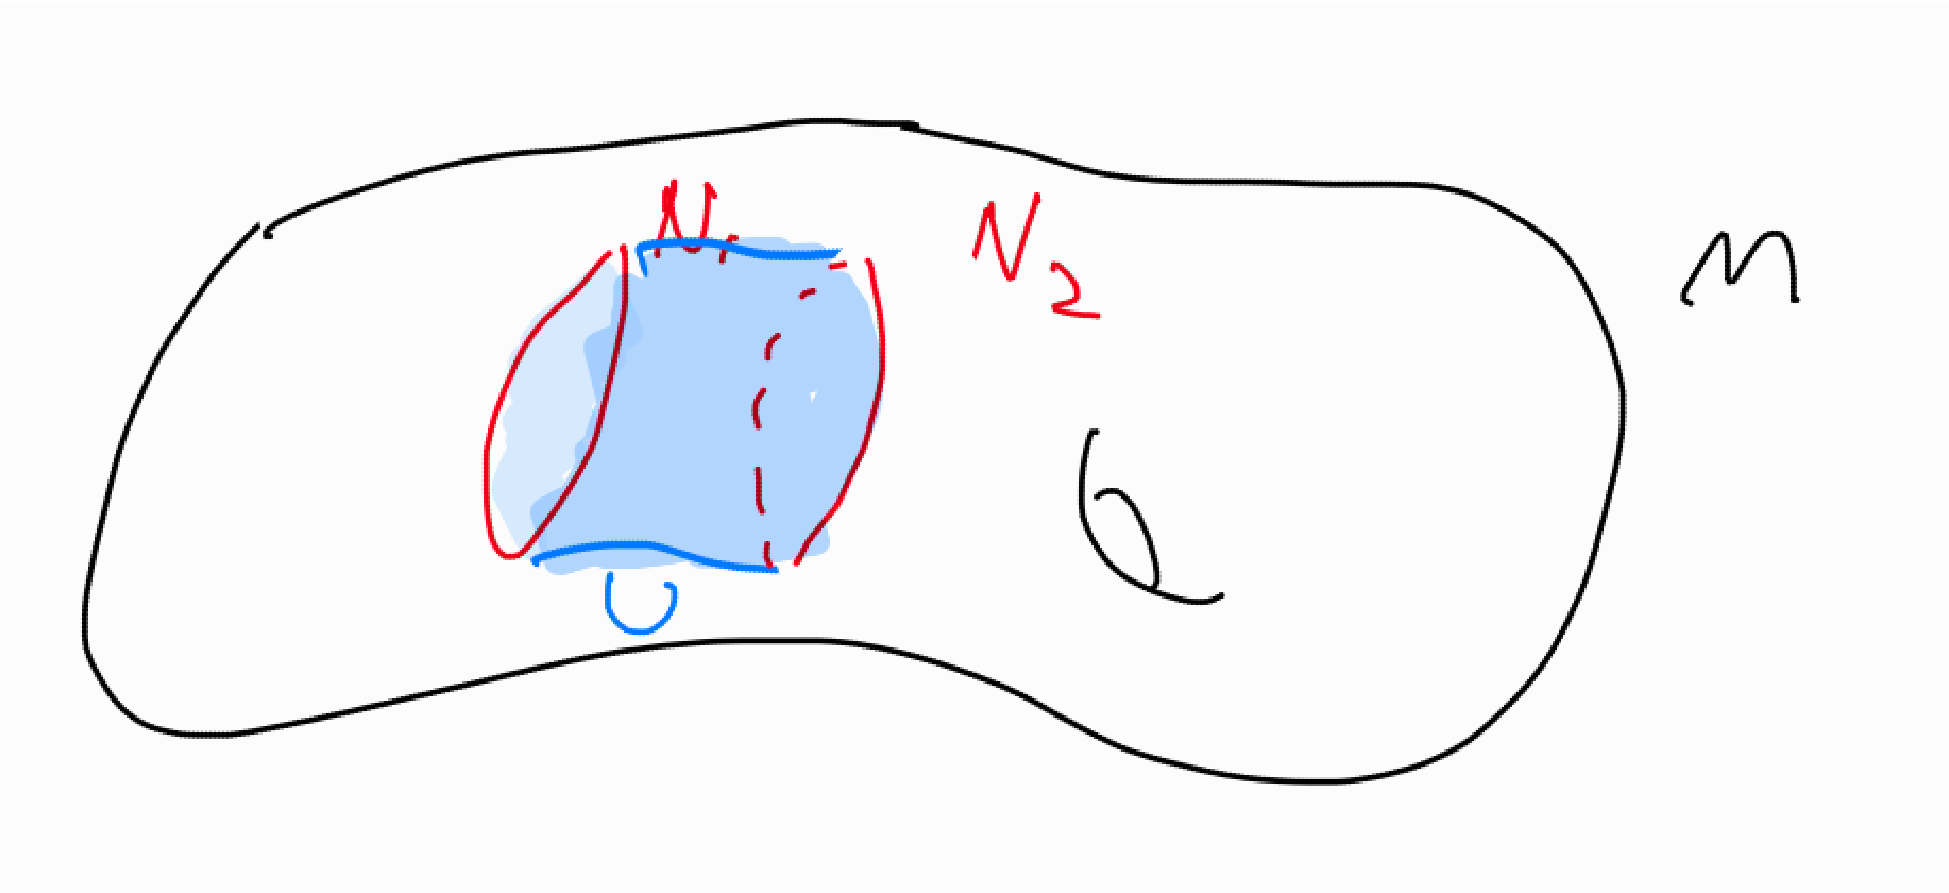
\includegraphics[width=0.62\textwidth]{figures/fig5_1.png}\\[2pt]
  {\small 图 5.1：$M$ 内两个“相近”的子流形 $N_1$ 与 $N_2$。}
\end{center}

\begin{proposition}{5.15}
  若 $p$-形式 $\omega$ 满足 $d\omega=0$，则对 $M$ 的两个“相近”的 $p$ 维子流形 $N_1$ 与 $N_2$，有 $\int_{N_1}\omega=\int_{N_2}\omega$。这里 $N_1$ 与 $N_2$ 称为“相近”的，是指存在 $(p+1)$ 维子流形 $U$ 使 $\partial U=N_1\sqcup\ol{N_2}$。
\end{proposition}

图 5.1 是“相近”这一概念的图示；记号 $\sqcup$ 表示不交并，$\ol{N_2}$ 上方的横线表示定向反转。注意，“相近”这一术语只是为本命题临时引入，并非标准术语。这里本该使用同调这一概念，但它的定义相当复杂，要推迟一阵子。

证明极其简单：
\begin{equation}
  \int_{N_1}\omega-\int_{N_2}\omega=\int_{\partial U}\omega=\int_U d\omega=0.
  \tag{5.37}
\end{equation}

这促使我们作以下定义。

\begin{definition}{5.16}
  $p$-形式 $\omega$ 在 $d\omega=0$ 时称为闭的；若它对某个 $(p-1)$-形式 $\eta$ 有形如 $\omega=d\eta$ 的表达式，则称为恰当的。
\end{definition}

由于 $d^2=0$，有

% [原文 p.81]
\begin{proposition}{5.17}
  恰当形式自动是闭的。
\end{proposition}

现在可以在两个闭 $p$-形式之间引入等价关系：若 $\omega_1-\omega_2=d\eta$ 对某个 $(p-1)$-形式 $\eta$ 成立，则定义 $\omega_1\sim\omega_2$。

\begin{definition}{5.18}
  闭 $p$-形式 $\omega$ 的等价类 $[\omega]$ 称为它的上同调类。所有这类上同调类的空间记作 $H^p_{\mathrm{dR}}(M)$。这就是 $M$ 的 de Rham 上同调群。
\end{definition}

注意，虽然它被称为“群”，它其实只是 $\R$ 上的向量空间。

前面关于 $p$-形式在 $p$ 维子流形上积分的讨论蕴含：

\begin{proposition}{5.19}
  上同调类 $[\omega]\in H^p_{\mathrm{dR}}(M)$ 在 $M$ 的 $p$ 维闭子流形 $N$ 上的积分良定义。而且，上同调类 $[\omega]$ 在两个“相近”的子流形 $N_1$ 与 $N_2$ 上的积分相同。
\end{proposition}

特别地，若 $[\omega]$ 满足存在 $N$ 使 $\int_N\omega\ne0$，则不存在 $\eta$ 使 $\omega=d\eta$。这也说明 $N$ 不是任何 $(p+1)$ 维子流形 $U$ 的边界，因此 $N$ 保证在 $M$ 中“非平凡”。

回忆给定映射 $f:X\to Y$，有拉回映射 $f^*:\Omega^p(Y)\to\Omega^p(X)$。它诱导映射 $f^*:H^p_{\mathrm{dR}}(Y)\to H^p_{\mathrm{dR}}(X)$，我们也称之为拉回。这显然是两个向量空间之间的线性映射。由此容易推出：

\begin{proposition}{5.20}
  若 $X$ 与 $Y$ 微分同胚，则 $H^p_{\mathrm{dR}}(X)$ 与 $H^p_{\mathrm{dR}}(Y)$ 同构。
\end{proposition}

\begin{proposition}{5.21}
  对紧的 $M$，$H^p_{\mathrm{dR}}(M)$ 是有限维的。
\end{proposition}

注意，闭 $p$-形式的空间与恰当 $p$-形式的空间都是函数空间，通常无限维。它们的“差”是有限维的，这是个有趣的事实，我们无法在此证明。

与同伦不同，de Rham 上同调群是可计算的：只要用坐标卡描述流形，就有算法计算它，尽管这里不能细说。这使上同调群成为研究流形拓扑的有用对象。

上同调群还有另一种结构。为此，设 $\alpha$ 与 $\beta$ 分别是 $p$-形式与 $q$-形式。当 $d\alpha=0$、$d\beta=0$ 时，有
\begin{equation}
  d(\alpha\wedge\beta)=(d\alpha)\wedge\beta+(-1)^p\alpha\wedge d\beta=0.
  \tag{5.38}
\end{equation}
又当 $\alpha=d\eta$ 时，
\begin{equation}
  \alpha\wedge\beta=d(\eta\wedge\beta).
  \tag{5.39}
\end{equation}
这意味着

% [原文 p.82]
\begin{proposition}{5.22}
  取两个上同调类 $[\alpha]\in H^p_{\mathrm{dR}}(M)$、$[\beta]\in H^q_{\mathrm{dR}}(M)$，构成 $[\alpha\wedge\beta]\in H^{p+q}_{\mathrm{dR}}(M)$，这一操作给出良定义的双线性乘法
  \begin{equation}
    H^p_{\mathrm{dR}}(M)\times H^q_{\mathrm{dR}}(M)\to H^{p+q}_{\mathrm{dR}}(M).
    \tag{5.40}
  \end{equation}
\end{proposition}

\takeaway{本节用闭形式与恰当形式定义 de Rham 上同调 $H^p_{\mathrm{dR}}(M)=Z^p(M)/B^p(M)$：$d^2=0$ 保证恰当形式必闭，商去恰当形式后，积分只依赖上同调类，而楔积在商上给出上积。}

\section{de Rham 上同调的例子}

我们至少给出一些非平凡的 de Rham 上同调类的例子。

\begin{proposition}{5.23}
  $H^0_{\mathrm{dR}}(M)=\R^k$，其中 $k$ 是 $M$ 的连通分支数。
\end{proposition}

要看出这一点，注意不存在恰当的 0-形式，因为一开始就没有 $-1$-形式。闭 0-形式是满足 $df=\sum_i\frac{\partial f}{\partial x^i}dx^i=0$（在每一点）的函数 $f$。这意味着 $f$ 的所有偏导数在 $M$ 的每一点都为零。因此 $f$ 局部常值，由在每个连通分支上指定一个常数决定。

\begin{example}{5.24}
  $H^p_{\mathrm{dR}}(S^n)$ 由下式给出：
  \[
    H^p_{\mathrm{dR}}(S^n)=
    \begin{cases}
      \R & (p=0),\\
      0 & (p=1,\dots,n-1),\\
      \R & (p=n).
    \end{cases}
  \]
  我们从 $n=1$ 开始。用 $0\le\theta\le2\pi$ 参数化 $S^1$。$p=0$ 的一般情形上面已讨论过。那么取 $p=1$。1-形式是 $g:=g(\theta)d\theta$，它自动满足 $dg=0$。假定这样的 $g(\theta)$ 由 $df=f'(\theta)d\theta$ 给出。这意味着 $g(\theta)=f'(\theta)$，即 $f(\theta)=c+\int_0^\theta g(t)dt$。$f$ 是圆上的函数，因此 $f(0)=f(2\pi)$。这意味着 $g(\theta)d\theta$ 恰当，当且仅当 $\int_0^{2\pi}g(\theta)d\theta=0$。注意，右边不过是 $\int_{S^1}g$。因此，两个 1-形式 $g_1$ 与 $g_2$ 满足 $[g_1]=[g_2]$，当且仅当 $\int_{S^1}g_1=\int_{S^1}g_2$。这意味着 $H^1_{\mathrm{dR}}(S^1)=\R$。
  
  对一般的 $n$，我只给出该陈述的一个粗略验证。取 $p$ 维闭子流形 $N\subset S^n$，考虑 $\int_N\omega$。当 $0<p<n$ 时，总可以在 $S^n$ 内收缩 $N$，找到 $U\subset S^n$ 使 $\partial U=N$。于是
  \begin{equation}
    \int_N\omega=\int_U d\omega=0.
    \tag{5.41}
  \end{equation}
  这与 $0<p<n$ 时 $H^p_{\mathrm{dR}}(S^n)=0$ 相容。对 $p=n$，上同调类 $[\omega]$ 由 $\int_{S^n}\omega$ 探测；注意 $S^n$ 不能在 $S^n$ 内收缩，所以 $\int_{S^n}\omega$ 可以非零，这没有问题。
\end{example}

\begin{example}{5.25}
  $H^p_{\mathrm{dR}}(\CP^n)$ 由下式给出：
  \[
    H^p_{\mathrm{dR}}(\CP^n)=
    \begin{cases}
      \R & (p:\text{偶}),\\
      0 & (p:\text{奇}).
    \end{cases}
  \]
  此外，记 $H^2_{\mathrm{dR}}(\CP^n)$ 的一个非平凡元素为 $c$，则 $c^k\in H^{2k}_{\mathrm{dR}}(\CP^n)$ 也非平凡。因此作为代数，有
  \[
    \bigoplus_p H^p_{\mathrm{dR}}(\CP^n)=\R[c]/(c^{n+1}).
  \]
\end{example}

% [原文 p.83]
考虑由
\begin{equation}
  [1:z_2:z_3:\cdots:z_{n+1}]
  \tag{5.42}
\end{equation}
与
\begin{equation}
  [w_1:1:w_3:\cdots:w_{n+1}]
  \tag{5.43}
\end{equation}
分别给出的两张坐标卡。回忆坐标之间的关系为 $w_i=z_i/z_2$，约定 $z_1=1$、$w_2=1$。还有别的坐标卡，但可以用同样的方式处理。

考虑定义在第一张坐标卡上的 1-形式 $A_{(z)}$，它由
\begin{equation}
  A_{(z)}=\frac{1}{2i}\frac{\sum_a(z_a\,d\bar z_a-\bar z_a\,dz_a)}{1+\sum_a|z_a|^2}.
  \tag{5.44}
\end{equation}
给出。类似地，考虑定义在第二张坐标卡上的
\begin{equation}
  A_{(w)}=\frac{1}{2i}\frac{\sum_a(w_a\,d\bar w_a-\bar w_a\,dw_a)}{1+\sum_a|w_a|^2}.
  \tag{5.45}
\end{equation}
在两坐标卡的交叠上，简短的计算表明
\begin{equation}
  A_{(z)}=A_{(w)}+\frac{1}{2i}\Bigl(\frac{dw_1}{w_1}-\frac{d\bar w_1}{\bar w_1}\Bigr)=A_{(w)}+d\theta_1,
  \tag{5.46}
\end{equation}
其中我们引入了 $w_1=r_1e^{i\theta_1}$。因此 $A_{(z)}$ 在轨迹 $w_1=0$ 附近并没有良好定义。但上式也表明，在交叠上有
\begin{equation}
  dA_{(z)}=dA_{(w)}.
  \tag{5.47}
\end{equation}
利用这一点，定义 2-形式 $\omega$：在第一张坐标卡上取 $\omega:=dA_{(z)}/(2\pi)$，在第二张坐标卡上取 $\omega:=dA_{(w)}/(2\pi)$。由于式 (5.47)，$\omega$ 处处良定义，且 $d\omega=0$。显式地，在第一张坐标卡上有
\begin{equation}
  \omega=\frac{1}{2\pi}\frac{1}{i}\left(
  \frac{\sum_a dz_a\wedge d\bar z_a}{1+\sum_a|z_a|^2}
  -\frac{(\sum_a\bar z_a\,dz_a)\wedge(\sum_a z_a\,d\bar z_a)}{(1+\sum_a|z_a|^2)^2}
  \right).
  \tag{5.48}
\end{equation}

下面要证明，$\omega^m$ 对 $m=0,\dots,n$ 是非平凡的上同调类，办法是在合适的 $2m$ 维子流形上积分它们。现在，$\CP^n$ 中由
\begin{equation}
  \{[z_1:z_2:\cdots:z_{n+1}]\mid z_{m+2}=z_{m+3}=\cdots=z_{n+1}=0\}
  \tag{5.49}
\end{equation}
给出的子空间是 $\CP^m$。我们对 $m$ 作归纳计算。对 $m=1$，$\CP^1$ 只用 $z:=z_2$ 参数化。需要计算
\begin{equation}
  \int_{\CP^1}\omega=\int\frac{1}{2\pi}\frac{1}{i}\frac{dz\wedge d\bar z}{(1+|z_2|^2)^2}.
  \tag{5.50}
\end{equation}

% [原文 p.84]
这可以显式算出为 $1$，但为使归纳过程更清楚，我们改写成
\begin{equation}
  \int_{\CP^1}\omega=\int_{z,\bar z}dA_{(z)}=\oint_{|z|=R}A_{(z)}
  =\oint_{|w|=1/R}\Bigl(A_{(w)}+\frac{d\theta}{2\pi}\Bigr).
  \tag{5.51}
\end{equation}
其中最后一个等号把坐标卡从第一张（用 $z:=z_2$ 参数化）换到第二张（用 $w:=w_1$ 参数化）。由于 $A_{(w)}$ 在第二张坐标卡上良定义，它在 $|w|=1/R$ 上的积分在 $R\to\infty$ 时消失，只剩下第二项，给出
\begin{equation}
  =\oint\frac{d\theta_1}{2\pi}=1.
  \tag{5.52}
\end{equation}

对 $m>1$，做法类似。注意在第一张坐标卡上 $\omega^m=d(A_{(z)}\omega^{m-1})$。第一张坐标卡由 $z_2,\dots,z_{m+1}$ 参数化，因此拓扑是 $\C^m=\R^{2m}$。它在无穷远处有渐近边界 $S^{2m-1}$。于是有
\begin{equation}
  \int_{\CP^m}\omega^m=\int_{\C^m}d(A_{(z)}\omega^{m-1})=\int_{S^{2m-1}}A_{(z)}\omega^{m-1},
  \tag{5.53}
\end{equation}
其中最后的积分是在第一张坐标卡的渐近边界 $S^{2m-1}$ 上。

现在，第一张坐标卡在 $\CP^m$ 内的补集是轨迹
\begin{equation}
  \{[0:z_2:\cdots:z_{m+1}]\in\CP^m\}\simeq\CP^{m-1}.
  \tag{5.54}
\end{equation}
因此，渐近边界 $S^{2m-1}$ 是 $\CP^{m-1}$ 上的 $S^1$ 纤维丛。我们的想法是先在纤维 $S^1$ 上对 $A_{(z)}\omega^{m-1}$ 积分，再把结果在 $\CP^{m-1}$ 上积分。为看出 $S^1$ 上的积分，转到第二张坐标卡比较方便；在第二张坐标卡中，第一张坐标卡的渐近边界位于 $|w_1|=1/R$，其中 $R$ 很小。于是有
\begin{equation}
  \int_{\CP^m}\omega^m=\oint_{\{|w_1|=1/R\}\cap\CP^m}\Bigl(A_{(w)}+\frac{d\theta_1}{2\pi}\Bigr)\omega^{m-1}.
  \tag{5.55}
\end{equation}
现在 $A_{(w)}$ 在 $w_1=0$ 处性态良好，因此它在小圆 $|w_1|=1/R$ 上的积分为零。于是只剩下来自 $d\theta_1/(2\pi)$ 的贡献，得到
\begin{equation}
  \int_{\CP^m}\omega^m=\oint\frac{d\theta_1}{2\pi}\int_{\CP^{m-1}}\omega^{m-1}
  =\int_{\CP^{m-1}}\omega^{m-1}.
  \tag{5.56}
\end{equation}
反复这样做，发现它等于 $1$。

\takeaway{本节算出两个基本例子：$H^p_{\mathrm{dR}}(S^n)$ 只在 $p=0,n$ 非零；$H^p_{\mathrm{dR}}(\CP^n)$ 由 $c=[\omega]$ 生成，$c^{n+1}=0$，并以 $\int_{\CP^m}\omega^m=1$ 说明 $\omega$ 不是恰当形式。}

\section{联络与 Maxwell 场}

上面我们看到，在 $M=\R^3$ 上，向量势与磁场强度的关系为 $B=dA$，其中 $A=A_xdx+A_ydy+A_zdz$，$B=B_xdy\wedge dz+B_ydz\wedge dx+B_zdx\wedge dy$。在更复杂的流形上，磁场 $B$ 仍是 2-形式，但向量势 $A$ 并不完全是一个 1-形式。

% [原文 p.85]
为说明这一点，我们从磁场中电荷为 $q$ 的带电粒子的哈密顿量出发，它由
\begin{equation}
  H=\frac{1}{2m}\sum_{a=1,2,3}\Bigl(-i\hbar\frac{\partial}{\partial x^a}-qA^{\mathrm{SI}}_a\Bigr)^2
  \tag{5.57}
\end{equation}
给出，作用在波函数 $\psi$ 上。规范变换
\begin{equation}
  A^{\mathrm{SI}}_a\mapsto\tilde A^{\mathrm{SI}}_a:=A^{\mathrm{SI}}_a+\frac{\partial\chi}{\partial x^a}
  \tag{5.58}
\end{equation}
需要补充波函数的变换
\begin{equation}
  \psi\mapsto\tilde\psi=e^{iq\chi/\hbar}\psi.
  \tag{5.59}
\end{equation}
的确，可以验证
\begin{equation}
  \Bigl(-i\hbar\frac{\partial}{\partial x^a}-q\tilde A^{\mathrm{SI}}_a\Bigr)e^{iq\chi/\hbar}\psi
  =e^{iq\chi/\hbar}\Bigl(-i\hbar\frac{\partial}{\partial x^a}-qA^{\mathrm{SI}}_a\Bigr)\psi
  \tag{5.60}
\end{equation}
因此规范变换后的哈密顿量
\begin{equation}
  \tilde H=\frac{1}{2m}\sum_{a=1,2,3}\Bigl(-i\hbar\frac{\partial}{\partial x^a}-q\tilde A^{\mathrm{SI}}_a\Bigr)^2
  \tag{5.61}
\end{equation}
与原哈密顿量 $H$ 共轭：
\begin{equation}
  \tilde H=e^{iq\chi/\hbar}He^{-iq\chi/\hbar},
  \tag{5.62}
\end{equation}
从而本征值不变。

现在可以把式 (5.59) 认作复线丛 $L\to M$ 在 $M$ 的两张坐标卡 $U$ 与 $V$ 之间的粘合规则：
\begin{equation}
  U\times\C\ni(b,\psi(b))\mapsto(b,\tilde\psi(b))=(b,g(b)\psi(b))\in V\times\C,
  \tag{5.63}
\end{equation}
其中 $g:U\cap V\to U(1)=\{|z|=1\}$，$g(b)=e^{iq\chi(b)/\hbar}$。现在考虑
\begin{equation}
  D\psi:=(d-iA)\psi=\sum_a\Bigl(\frac{\partial}{\partial x^a}-iA_a\Bigr)\psi\,dx^a
  \tag{5.64}
\end{equation}
与
\begin{equation}
  D\tilde\psi:=(d-i\tilde A)\tilde\psi=\sum_a\Bigl(\frac{\partial}{\partial x^a}-i\tilde A_a\Bigr)\tilde\psi\,dx^a,
  \tag{5.65}
\end{equation}
其中
\begin{equation}
  A=\sum_aA_a\,dx^a,\qquad A_a:=\frac{q}{\hbar}A^{\mathrm{SI}}_a,
  \tag{5.66}
\end{equation}

% [原文 p.86]
对带波浪号的版本同理，于是
\begin{equation}
  \tilde A_a=A_a-ig^{-1}\frac{\partial g}{\partial x^a},
  \tag{5.67}
\end{equation}
或等价地
\begin{equation}
  \tilde A=A-ig^{-1}dg.
  \tag{5.68}
\end{equation}
我们于是发现
\begin{equation}
  D\tilde\psi=(d+i\tilde A)\tilde\psi=g(b)(d+iA)\psi=g(b)D\psi,
  \tag{5.69}
\end{equation}
这意味着，坐标卡 $U$ 上的 $D\psi$ 与坐标卡 $V$ 上的 $D\tilde\psi$ 合起来定义 $(L\otimes T^*M)\to M$ 的一个截面。
% [Tutor Note: 原文式 (5.69) 的符号与式 (5.64)、(5.65) 的约定不一致：按 (5.64) 的 $D=(d-iA)$，此处应为 $d-i\tilde A$ 与 $d-iA$。照录原文，已登记为笔误。]

\begin{definition}{5.26}
  复线丛 $L\to M$（或等价地，主 $U(1)$ 丛 $P\to M$）上的联络，是 $M$ 的各坐标卡 $U$ 上的一族 1-形式 $A_{(U)}$，使得在交叠 $U\cap V$ 上有
  \begin{equation}
    A_{(V)}=A_{(U)}-ig^{-1}dg,
    \tag{5.70}
  \end{equation}
  其中线丛由粘合规则
  \begin{equation}
    U\times\C\ni(b,\psi(b))\mapsto(b,\tilde\psi(b))=(b,g(b)\psi(b))\in V\times\C
    \tag{5.71}
  \end{equation}
  构成，$g:U\cap V\to U(1)$。
\end{definition}

我们通常不写出下标 $A_{(U)}$，直接称它们为 $A$。

令每张坐标卡 $U$ 上 $F_{(U)}=dA_{(U)}$。于是有
\begin{equation}
  F_{(V)}=dA_{(V)}=dA_{(U)}-i\,d(g^{-1}dg)=F_{(U)}.
  \tag{5.72}
\end{equation}
（要看出上面最后一个等号，注意至少在局部 $g=e^{i\theta(b)}$ 对某个函数 $\theta(b)$ 成立。于是 $-ig^{-1}dg=d\theta$，故 $d(g^{-1}dg)=d^2\theta=0$。）无论如何，这意味着 $F_{(U)}$ 与 $F_{(V)}$ 在交叠 $U\cap V$ 上一致，并拼成 $M$ 上的 2-形式。

\begin{notation}{5.27}
  给定 $U(1)$ 联络 $A$，在各坐标卡上局部由 $F=dA$ 给出的 2-形式 $F$，称为该联络的曲率。
\end{notation}

当我们研究 $\CP^n$ 的上同调时，用到了式 (5.48) 定义的 $\omega$，它用到各坐标卡上定义的 1-形式 $A_{(z)}$、$A_{(w)}$，见 (5.44)、(5.45)、(5.46)。现在我们认出它们定义了 $\CP^n$ 上的 $U(1)$ 联络，其中粘合函数 $g:U\cap V\to U(1)$ 由 $g=e^{i\theta_1}$ 给出。于是 2-形式 $\omega$ 由 $\omega=F/(2\pi)$ 给出，其中 $F$ 是曲率 2-形式。那里的 2-形式 $\omega$ 是闭的。这是普遍现象：

\begin{proposition}{5.28}
  曲率 2-形式是闭的，$dF=0$。
\end{proposition}

这可以在每张坐标卡上容易地验证：$dF=d^2A=0$。这并不意味着 $F$ 总是恰当的；要使 $F$ 恰当，需要找到整体定义在 $M$ 上的 1-形式 $\eta$，使 $F=d\eta$。

曲率 2-形式的一个重要特征是：

% [原文 p.87]
\begin{proposition}{5.29}
  曲率 2-形式 $F$ 在 $M$ 的 2 维闭子流形 $N$ 上的积分是 $2\pi$ 的整数倍。
\end{proposition}

对 $N=S^2$ 证明一下。用两张坐标卡 $U$ 与 $V$ 覆盖 $S^2$，分别对应北半球与南半球，于是 $U$ 与 $V$ 有公共边界，即赤道。$F$ 在 $U$ 上由 $F=dA_{(U)}$ 给出，在 $V$ 上由 $F=dA_{(V)}$ 给出。于是有
\begin{equation}
  \int_{S^2}F=\int_UF+\int_VF=\int_{\partial U}A_{(U)}+\int_{\partial V}A_{(V)}
  =\int_{S^1}(A_{(U)}-A_{(V)})=\int_{S^1}-ig^{-1}dg.
  \tag{5.73}
\end{equation}
其中 $g:S^1\to U(1)$ 是从赤道到群 $U(1)$ 的映射。

用 $0\le s<2\pi$ 参数化源 $S^1$，用 $z=e^{i\theta}$ 参数化靶 $U(1)$。则 $g(s)=e^{i\theta(s)}$，且
\begin{equation}
  \int_{S^2}F=\int_0^{2\pi}\frac{d\theta}{ds}ds=2\pi n,
  \tag{5.74}
\end{equation}
其中 $n$ 是映射 $g:S^1\to U(1)$ 的缠绕数。这个整数 $n$ 也称 Chern 数。

这一事实最早由 Dirac 在物理侧发现 [Dir31]。回忆一下，换到 SI 单位制要用
\begin{equation}
  F^{\mathrm{SI}}=\frac{\hbar}{q}F,\qquad A^{\mathrm{SI}}=\frac{\hbar}{q}A.
  \tag{5.75}
\end{equation}
还要回忆，在 $\R^3$ 上 $F=B_xdy\wedge dz+B_ydz\wedge dx+B_zdx\wedge dy$，因此 $F$ 在 2-球面 $S^2$ 上的积分是通过球面的磁通量。我们得出：

\begin{proposition}{5.30}
  通过 2-球面 $S^2$ 的磁通量以 $2\pi\hbar/e$ 为单位量子化，其中 $e$ 是电子的电荷。
\end{proposition}

这就是 Dirac 量子化条件。

\textbf{附注 5.31.} 两个带最小电荷的电粒子相距 $r$ 时，库仑力为
\begin{equation}
  F=\frac{e^2}{4\pi\epsilon_0r^2}.
  \tag{5.76}
\end{equation}
类似地，两个带最小磁荷的磁单极子相距 $r$ 时，库仑力为
\begin{equation}
  F=\frac{g^2}{4\pi\mu_0r^2},
  \tag{5.77}
\end{equation}
其中 $g=2\pi\hbar/e$，如上所述。于是发现比值
\begin{equation}
  \frac{\text{相距 }r\text{ 的单位电荷之间的力}}{\text{相距 }r\text{ 的单位磁荷之间的力}}
  \tag{5.78}
\end{equation}
与距离 $r$ 无关，且等于
\begin{equation}
  =\frac{\mu_0}{\epsilon_0}\frac{e^4}{(2\pi\hbar)^2}
  =4\Bigl(\frac{e^2}{4\pi\epsilon_0\hbar c}\Bigr)^2\sim0.0002\cdots,
  \tag{5.79}
\end{equation}

% [原文 p.88]
最后一行用了 $\mu_0\epsilon_0=1/c^2$。括号中的组合
\begin{equation}
  \alpha=\frac{e^2}{4\pi\epsilon_0\hbar c}\sim\frac{1}{137},
  \tag{5.80}
\end{equation}
称为精细结构常数。\qedmark

\begin{center}
\begin{tabular}{cc}
\toprule
物理 & 数学\\
\midrule
Maxwell 场的拓扑 & 主 $U(1)$ 丛\\
向量势 & 联络\\
场强 & 曲率\\
磁通量 & Chern 数\\
\bottomrule
\end{tabular}\\[2pt]
{\small 表 3：术语翻译对照表}
\end{center}

本节末尾，还有几点说明：

\begin{itemize}
  \item 如你们所见，同一概念在物理与数学中名称不同。表 3 把它们列在一起。
  \item 曲率 2-形式 $F$ 是闭的，因此定义 de Rham 上同调群中的一个元素。它有特殊性质：$F/(2\pi)$ 在闭 2 维子流形上的积分总是整数。这促使我们寻找从一开始就用 $\Z$ 而非 $\R$ 定义的 de Rham 上同调类比物。这将把我们引向以一般阿贝尔群 $A$ 为系数的（上）同调概念，而不只是 $\R$ 与 $\Z$。
  \item 由于这个积分是整数，$F/(2\pi)$ 在各种 2 维子流形上的积分也不随 $U(1)$ 丛及其上联络的连续变化而改变。因此这些整数给出 $U(1)$ 丛的拓扑不变量。这促使我们寻找系统的方法来得到各种其他丛的拓扑不变量。这将把我们引向示性类理论。
  \item 在 $2+1$ 维系统中，霍尔电导 $\sigma$ 由有效作用量中正比于 $\sigma\int_MA\wedge F$ 的项刻画，其中 $A$ 是向量势，$F$ 是磁场。组合 $\int_MA\wedge F$ 称为 Chern--Simons 项。由于作为 1-形式的 $A$ 只在每张坐标卡上有定义，Chern--Simons 项的定义很微妙；这最终导致量子情形下霍尔电导 $\sigma$ 的量子化条件，从而给出整数量子霍尔效应的代数拓扑解释。我希望在本系列讲义结束前覆盖这个主题！
\end{itemize}

\clearpage
\takeaway{本节把 $U(1)$ 规范场翻译成线丛上的联络：向量势是联络，场强是曲率，磁通量是 Chern 数。曲率闭而不总是恰当，它在闭曲面上的积分量子化为 $2\pi$ 的整数倍，这就是 Dirac 量子化条件，也提示上同调应取整系数。}

\chapterreview{本章把微分形式、外微分与积分组织成 de Rham 上同调。§5.1 定义 $p$-形式与 $d$，由 $d^2=0$ 读出梯度、旋度、散度之间的关系。§5.2 引入拉回，证明一般 Stokes 定理，并在 $\R^3$ 上收回经典公式。§5.3 定义闭形式与恰当形式，说明积分只依赖上同调类，并给出上积。§5.4 计算球面与复射影空间的上同调。§5.5 把规范势、场强、磁通量与联络、曲率、Chern 数对应起来，由 Dirac 量子化条件提示系数应取 $\Z$。}
